\chapter{Complexidade Computacional}

% Funções de complexidade, que satisfazem aos axiomas de Blum
\newcommand{\PhiDT}{{\mathcal{T}}} % Tempo determinístico
\newcommand{\PhiDS}{{\mathcal{S}}} % Espaço determinístico
\newcommand{\PhiNT}{{\mathcal{N\!T}}} % Tempo não-determinístico
\newcommand{\PhiNS}{{\mathcal{N\!S}}} % Espaço não-determinístico

\emph{Complexidade} é a quantidade de recursos
que uma máquina de Turing gasta
para computar determinada função
ou para decidir pertinência a uma linguagem
\cite[p. 285]{HopcroftUllman1979}.
Os recursos mais importantes para a teoria de complexidade computacional
são o espaço e o tempo,
tanto determinísticos como não"-determinísticos.

Embora seja possível trabalhar com estas medidas diretamente,
muitos resultados para uma medida
possuem análogos em outra medida.
Para simplificar a exposição,
escolhemos iniciar,
na seção \ref{axiomas_blum},
uma discussão sobre teoria de complexidade axiomática,
e definir as medidas padrão na seção \ref{medidas_padrao}.

\section{Teoria de Complexidade Axiomática: Axiomas de Blum}
\label{axiomas_blum}

(Utilizaremos a definição provida por
\citeonline[p. 156]{Papadimitriou1994}.)

Dada uma máquina de Turing $M$
e uma palavra $x$,
denotaremos por $M(x)$ a ``saída''
de $M$ quando lhe é dado $x$ na entrada.

\begin{definition}
    Uma \emph{medida de complexidade}
    é uma função $\Phi$ que satisfaz aos seguintes axiomas:
    \footnotemark
    \begin{enumerate} [label=\textbf{Axioma \arabic*}, ref=\arabic*, align=left]
        \item
            \label{blum_def}
            $\Phi(M, x)$ está definido
            se, e somente se,
            $M(x)$ está definido.
        \item
            \label{blum_rec}
            Dados $M$, $x$ e $k$,
            é decidível se $\Phi(M, x) = k$.
    \end{enumerate}

    \footnotetext{
        A definição usual dos axiomas de Blum
        (encontrada, por exemplo,
        no texto de \citeonline[p. 313]{HopcroftUllman1979}
        e no próprio artigo original de \citeonline[p. 3]{Blum1967})
        aparece no contexto de computadores de funções de inteiros.
        Seja $M_1, M_2, \dots$ uma enumeração de máquinas de Turing.
        Consideraremos que a máquina $M_i$
        computa a função recursiva parcial $\phi_i$.
        Uma medida de complexidade é uma lista de funções
        $\{\hat \Phi_1, \hat \Phi_2, \dots\}$
        que satisfaz os seguintes axiomas:

        \begin{enumerate} [label=Axioma \arabic*', ref=\arabic*', align=left]
            \item
                \label{blum_def_orig}
                $\hat \Phi_i(n)$ está definido
                se, e somente se,
                $\phi_i(n)$ está definido.
            \item
                \label{blum_rec_orig}
                A função $R(i, n, m)$,
                definida como $1$ se $\hat \Phi_i(n) = m$,
                e $0$ em caso contrário,
                é recursiva.
        \end{enumerate}

        As duas definições são análogas.
        O valor $\hat \Phi_i(n)$ corresponde a $\Phi(M_i, 0^n)$.
        O axioma \ref{blum_def} corresponde ao axioma \ref{blum_def_orig},
        enquanto que a decidibilidade exigida pelo axioma \ref{blum_rec}
        é expressada pela função $R$ no axioma \ref{blum_rec_orig}.
    }
\end{definition}

O axioma \ref{blum_rec}
nos dá um semialgoritmo para calcular $\Phi(M, x)$.
Entretanto, pelo axioma \ref{blum_def},
não podemos ir muito além disso,
pois $M(x)$ não está definido para todo $M$ e $x$.
De fato, sequer podemos decidir se $\Phi(M, x)$ existe.

\begin{example}
    \simbolo{$\PhiDT$}{Complexidade de Tempo}
    A \emph{complexidade de tempo},
    que denotaremos por $\PhiDT$,
    é a função que diz quantos movimentos
    uma máquina de Turing faz até retornar uma resposta.
    Isto é,
    \begin{equation*}
        \PhiDT(M, x) = \begin{cases}
            k, & \text{
                \parbox{0.6\textwidth}{
                    se $M$ executa exatamente $k$ passos em $x$ antes de parar.
                }
            } \\
            \text{indefinido}, & \text{
                \parbox{0.6\textwidth}{
                    caso $M$ nunca pare de computar $x$.
                }
            }
        \end{cases}
    \end{equation*}
    Para determinar se $\PhiDT(M, x) = k$,
    execute a máquina $M$ por $k$ passos
    e veja se é a primeira vez que
    $M$ atinge um estado aceitador.
    E, como $\PhiDT(M, x)$ só está definido se $M$ para ao computar $x$,
    $\PhiDT$ satisfaz aos dois axiomas de Blum.
\end{example}

\begin{example}
    \label{complexidade_espaco}
    \simbolo{$\PhiDS$}{Complexidade de Espaço}
    Para a \emph{complexidade de espaço},
    que denotaremos por $\PhiDS$,
    iremos assumir que $M$ possui uma fita somente"-leitura
    específica para a entrada.
    \begin{equation*}
        \PhiDS(M, x) = \begin{cases}
            k, & \text{
                \parbox{0.6\textwidth}{%
                    se $M$ lê, de alguma de suas fitas,
                    exatamente $k$ células
                    antes de parar.
                }
            } \\
            \text{indefinido}, & \text{
                \parbox{0.6\textwidth}{
                    se $M$ nunca parar ao computar $x$.
                }
            }
        \end{cases}
    \end{equation*}
    É fácil ver que o axioma \ref{blum_def} é satisfeito.
    Para o axioma \ref{blum_rec},
    o algoritmo é um pouco mais complicado.

    Comece executando $M$ em $x$.
    Caso $M$ extrapole $k$ células lidas
    em alguma de suas fitas,
    podemos retornar rejeitar.
    Caso contrário,
    existirá um número finito de configurações da máquina.
    Existem $|\Gamma|^k$ possíveis fitas com $k$ termos;
    $k+1$ possíveis posições da cabeça de leitura;
    $|Q|$ possíveis estados da máquina;
    e $l$ diferentes fitas.
    No total, existem, no máximo,
    \begin{equation*}
        (k+1) l |Q||\Gamma|^k
    \end{equation*}
    possíveis configurações.
    Portanto, se a máquina executar
    mais movimentos do que este número,
    significa que ela entrou em loop.
    Podemos retornar rejeitar.

    E, por último,
    caso $M$ pare,
    precisamos nos assegurar que,
    de fato,
    em alguma das fitas $k$ células foram lidas.
\end{example}

\begin{example}
    \simbolo{$\PhiNT$}{Complexidade de Tempo não"-determinística}
    \simbolo{$\PhiNS$}{Complexidade de Espaço não"-determinística}
    Podemos adaptar $\PhiDT$ e $\PhiDS$
    para aaaaaa máquinas de Turing não"=determinísticas.

    Para a complexidade de tempo não"-determinística,
    que denotaremos por $\PhiNT$,
    definiremos $\PhiNT(M, x)$
    como sendo a maior quantidade de movimentos
    tomadas por $M$ ao computar $x$
    dentre todas as escolhas de transições possíveis.

    Analogamente,
    para a complexidade de espaço não"-determinística,
    que denotaremos por $\PhiNS$,
    definiremos $\PhiNS(M, x)$
    como sendo a maior quantidade de células lidas
    em qualquer dos ramos da computação de $M$ em $x$.
    Aqui, precisamos tomar o mesmo cuidado que tomamos
    com $\PhiDS$ para demonstrar o axioma \ref{blum_rec}.
\end{example}

\begin{example}
    Escolher $\Phi(M, x) = 0$ para todo $M$ e $x$
    satisfaz ao axioma \ref{blum_rec},
    mas não ao axioma \ref{blum_def},
    pois $\Phi(M, x)$ está definida mesmo quando $M(x)$ não está.
    Já definir $\Phi(M, x) = |M(x)|$
    satisfaz ao axioma \ref{blum_def},
    mas não ao axioma \ref{blum_rec},
    pois poderíamos resolver o problema da parada:
    dada uma máquina $M$, podemos modificá"-la
    para apagar sua fita logo antes de parar.
    Então, para esta $M'$,
    $\Phi(M', x) = 0$ se, e somente se,
    a $M$ original para ao computar $x$.
    Estes dois exemplos mostram que os axiomas são independentes
    \cite[p. 3]{Blum1967}.
\end{example}

Podemos ver que as medidas $\PhiDT$ e $\PhiDS$ estão relacionadas.
Para ler uma posição da fita,
é necessário gastar ao menos uma unidade de tempo.
Ou seja,
\begin{equation*}
    \PhiDS(M, x) \leq \PhiDT(M, x).
\end{equation*}
E, de acordo com o raciocínio do exemplo \ref{complexidade_espaco},
para todo $M$ existe algum $c$ que
\begin{equation*}
    \PhiDT(M, x) \leq c^{\PhiDS(M, x)}.
\end{equation*}
De fato, podemos relacionar quaisquer duas medidas de complexidade.

\begin{theorem}
    \label{relacao_medidas}
    Dadas duas medidas de complexidade $\Phi$ e $\hat \Phi$,
    existe uma função recursiva $r$ tal que
    \begin{equation*}
        \Phi(M, x) \leq r( x, \hat \Phi(M, x))
    \end{equation*}
    para todo $M$ e quase todo $x$.
    \footnote{
        ``verdadeiro para quase todo $n$''
        significa que o predicado em questão
        é falso para apenas uma quantidade finida de números $n$.
    }
\end{theorem}

\begin{proof}
    Defina
    \begin{equation*}
        r( x, k ) = \max \{ \Phi(M, x) \ | \
            \text{A desrição de $M$ é mais curta que $|x|$}
            \text{ e }
            \hat \Phi(M, x) = k
        \}
    \end{equation*}
    Fixado $x$, existe um número finito de máquinas de Turing
    cuja descrição é menor que $|x|$.
    O conjunto na definição acima é um subconjunto desta lista.
    O predicado $\hat \Phi(M, x) = k$ é recursivo.
    Quando este predicado é verdadeiro,
    $M(x)$ está definido, pelo axioma \ref{blum_def},
    portanto $\Phi(M, x)$ também está definido.
    Concluímos que $r$ é recursiva.

    Agora, para todos os $x$ que são mais longos que a descrição de $M$,
    $\Phi(M, x)$ será um dos elementos do conjunto acima
    para $r( x, \hat \Phi(M, x)))$,
    portanto é menor ou igual a este número.
\end{proof}

\citeonline[p. 4]{Blum1967} demonstra uma versão ligeiramente mais forte
deste teorema.
Ele prova que $r$ pode ser tal que,
simultaneamente,
\begin{equation*}
    \Phi(M, x) \leq r( x, \hat \Phi(M, x))
\end{equation*}
e
\begin{equation*}
    \hat \Phi(M, x) \leq r( x, \Phi(M, x))
\end{equation*}
Podemos construir uma função dessas
pegando o máximo de duas funções obtidas
usando o teorema \ref{relacao_medidas}.

Observe que o teorema,
assim como provamos,
não pode ser fortalecido
para que $r$ seja uma função de apenas uma variável.
Considere $A$ uma máquina de Turing
que opere como um autômato finito.
$\PhiDT(A, x) = |x|$ para toda palavra $x$,
enquanto que $\PhiDS(A, x) = 1$ para toda palavra $x$.
\footnote{
    A complexidade de espaço não é $0$
    pois $A$ é obrigada a ler
    ao menos a célula inical da sua fita de trabalho,
    embora a máquina não use aquela célula.
}
Se $r$ pudesse depender apenas da segunda variável,
isto é, $r(x, m) = r'(m)$ para alguma função $r'$,
teríamos
\begin{align*}
    |x| &= \PhiDT(A, x) \\
        &\leq r(x, \PhiDS(A, x)) \\
        &= r(x, 1) \\
        &= r'(1)
\end{align*}
que é falso para todo $x$ suficientemente comprido.

Caso $r$ pudesse depender apenas da primeira variável,
isto é, $r(x, m) = r''(x)$ para alguma função $r''$,
teríamos, para todas as máquinas de Turing,
\begin{equation*}
    \PhiDT(M, x) \leq r''(x).
\end{equation*}
Mas, como $r''$ é recursiva
(pois $r$ o é),
podemos construir uma máquina que calcula $r''(x)$,
disperdiça $r''(x)$ movimentos,
e aceita a entrada.
Para esta $M'$,
\begin{equation*}
    \PhiDT(M', x) > r''(x),
\end{equation*}
contradizendo a equação anterior.

No parágrafo anterior,
construímos uma máquina de Turing
que deliberadamente desperdiça tempo
ao computar determinada função.
Utilizando alguns resultados da teoria de funções recursivas,
\citeonline[p. 4]{Blum1967} demonstrou que
é sempre possível desperdiçar recursos computacionais,
quaisquer que sejam estes recursos.

\begin{theorem}
    Sejam $f$ e $g$ duas funções recursivas totais,
    e $\Phi$ uma medida de complexidade.
    Então existe uma máquina de Turing $M$ que computa $f$
    tal que
    \begin{equation*}
        \Phi(M, x) \geq g(|x|)
    \end{equation*}
    para todo $x$.
\end{theorem}

Em outras palavras,
código ruim pode ser feito em qualquer linguagem.

\subsection{Classes de Complexidade}

\begin{definition}
    Dada uma medida de complexidade $\Phi$
    e uma função recursiva total
    $f: \mathbb N \rightarrow \mathbb N$,
    a \emph{classe de complexidade $f$} com relação a $\Phi$
    é o conjunto
    \begin{equation*}
        \mathcal C_\Phi(f) = \{ L(M) \ | \ \Phi(M, x) \leq f(|x|)
            \text{para quase todos os $x$}
        \}
    \end{equation*}
\end{definition}
Permitiremos que a complexidade de $M$
possa ser maior que $f$ para um número finito de elementos
para simplificar as demonstrações.

Embora faça sentido definir $\mathcal C_\Phi(f)$
para funções $f$ arbitrárias,
a exigência de $f$ ser recursiva total
torna as classes de complexidade
sucetíveis a argumentos por diagonalização.

Por exemplo,
podemos mostrar que
nenhuma classe de complexidade contém todas as linguagens recursivas.
Precisamos de um lema.

\begin{lemma}
    Existe um mapeamento bijetivo computável
    entre $\mathbb N$ e $\mathbb N \times \mathbb N$.
\end{lemma}

\begin{proof}
    Percorra o caminho descrito pelas setas na figura
    \ref{passeio_cantor}.

    \begin{figure}[h]
        \centering
        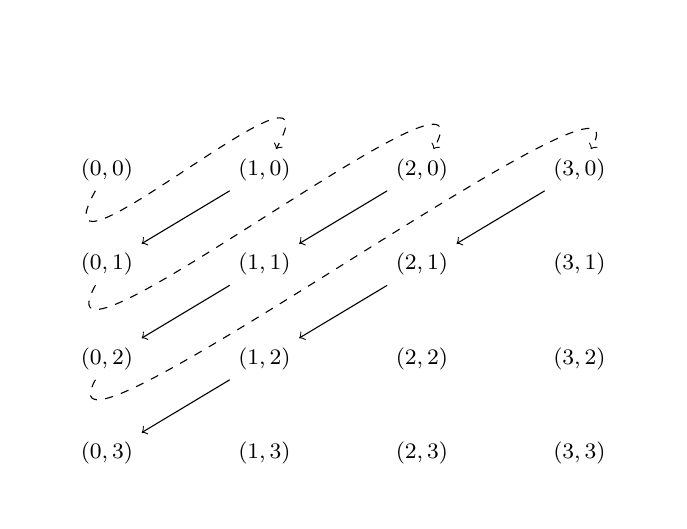
\begin{tikzpicture}
            \foreach \i in {0,...,3}
            \foreach \j in {0,...,3} {
                \node[font=\footnotesize]
                    (a\i\j) at (2*\i, -1.2*\j) {$(\i, \j)$};
            }

            \foreach \a/\b in {a00/a10, a01/a20, a02/a30} {
                \draw[->, dashed] (\a) .. controls
                +(-1,-1.8) and
                +(1, 1.8) .. (\b);
            }

            \foreach \a/\b in {
                a10/a01, a20/a11, a11/a02,
                a30/a21, a21/a12, a12/a03%
            } {
                \draw[->] (\a) -- (\b);
            }
        \end{tikzpicture}
        \caption{Passeio de Cantor.}
        \label{passeio_cantor}
    \end{figure}

    Em essência, primeiro enumeraremos todas os pares $(m, n)$
    para os quais $m + n = 0$,
    depois todos aqueles que $m + n = 1$,
    depois todos os que $m + n = 2$,
    e assim por diante.

    Esta técnica é conhecida como ``passeio de Cantor''
    \cite[p. 6]{CarnielliConiglioBianconi2006}.
\end{proof}

\begin{lemma}
    Existe uma função sobrejetora computavel
    $f: \mathbb N \rightarrow \mathbb N$
    tal que,
    para todo $y$,
    existem infinitos $x$ tais que $f(x) = y$.
\end{lemma}
\begin{proof}
    Considere $g$ como a função do lema anterior,
    e defina
    \begin{equation*}
        f(x) = y \quad \text{se $g(x) = (y, z)$.} \qedhere
    \end{equation*}
\end{proof}

\begin{lemma}
    Existe uma máquina de Turing $N$
    tal que $N(x)$ sempre está definido,
    e representa uma máquina de Turing,
    de forma que toda \emph{representação}
    de uma máquina de Turing
    é $N(x)$ para infinitamente muitos $x$.
    Isto é, $N$ produz todas as representações de máquinas de Turing
    infinitas vezes,
    conforme permitimos que $x$ tome valores arbitrários de $\Sigma^*$.
\end{lemma}

\begin{proof}
    Observe que existe uma bijeção computável
    entre palavras de $\Sigma^*$
    e números naturais.
    $N$ irá,
    dado um $x$,
    computar o número natural equivalente a ele
    e usar a função do lema anterior
    para gerar outro número.
    Então, $N$ irá converter este outro número
    novamente para uma palavra de $\Sigma^*$.

    Todas as palavras de $\Sigma^*$
    são representações de máquinas de Turing;
    portanto, esta palavra produzida é a máquina desejada.

    Como a função do lema anterior
    produz todos números naturais infinitas vezes
    (e $N$ é capaz de suprir todos os números naturais
    como entrada para aquela função),
    todas as representações de máquinas de Turing
    são produzidas por $N$ infinitas vezes.
\end{proof}

\begin{theorem}
    Seja $\mathcal C_\Phi(f)$ uma classe de complexidade
    com relação à $\Phi$.
    Então existe uma linguagem $L$
    que não pertence à esta classe de complexidade.
\end{theorem}

\begin{proof}
    Iremos construir linguagem $L$
    que discorda de todas as máquinas de Turing que gastam menos de
    $f(n)$ recursos ao computar uma palavra de tamanho $n$.

    Usaremos a máquina $N$ do lema anterior.
    Denotaremos por $M_x$
    a máquina de Turing que $N$ produz
    ao lhe ser dada a palavra $x$.
    Iremos pôr $x$ em $L$
    de acordo com o comportamento que $M_x$ tem ao computar $x$.
    Caso esta máquina encerre sua computação
    gastando no máximo $f(|x|)$ recursos,
    executaremos"-na até o final da computação
    e inverteremos o resultado:
    se $M_x$ aceita $x$, então $x \notin L$;
    se $M_x$ rejeita $x$, então $x \in L$.
    Caso $M_x$ exiga mais do que $f(|x|)$ recursos,
    coloque $x$ em $L$.
    \footnote{
        Este argumento é,
        de certa forma,
        uma versão limitada
        (por $f$)
        do problema da parada.
    }

    Em outras palavras,
    \begin{equation*}
        L = \{ x \ | \ \text{
            $M_x$ não aceita $x$ gastando menos de $f(|x|)+1$ recursos
        } \}
    \end{equation*}

    Determinar se $M_x$ computa $x$ usando no máximo $f(|x|)$ de recursos
    é equivalente a determinar se $\Phi(M_x, x) = k$
    para algum $k \leq f(|x|)$.
    Como $f(|x|)$ é computável
    e ``$\Phi(M_x, x) = k$'' é decidível
    (pelo axioma \ref{blum_rec}),
    esta verificação é realizável por uma máquina de Turing.
    Caso a resposta seja negativa
    ($M_x$ gasta mais do que $f(|x|)$ recursos ao computar $x$),
    já sabemos que $x$ está em $L$.
    Caso contrário,
    $\Phi(M_x, x)$ está definido;
    pelo axioma \ref{blum_def},
    $M_x(x)$ também está.
    Portanto, podemos executar $M_x$ em $x$
    e inverter a resposta.

    Podemos computar $M_x$ e executar a operação descrita no parágrafo anterior;
    isso garante que $L$ é recursiva.

    Suponha agora que alguma máquina $M$ reconheça $L$.
    $M$ é $M_x$ para infinitos $x$ diferentes.
    $M$ aceita todos esses $x$
    e precisa fazê"-lo gastando mais do que $f(|x|)$ recursos,
    caso contrário $L$ discordaria de $L(M)$ nesses pontos.
    Portanto, $\Phi(M, x) \geq f(|x|)$ para infinitos $x$.

    Ou seja, qualquer máquina que aceite $L$
    precisa gastar mais de $f(|x|)$ recursos para infinitos $x$,
    portanto o predicado ``$\Phi(M, x) \leq f(|x|)$ para quase todos os $x$''
    não pode ser verdadeiro.
    Portanto,
    \begin{equation*}
        L \notin \mathcal C_\Phi(f). \qedhere
    \end{equation*}
\end{proof}

\subsection{Teorema da União}

Na seção \ref{classes_complexidade},
iremos definir algumas classes de complexidade computacional
como sendo a união de infinitas classes de complexidade.
O teorema da união diz que,
sob condições apropriadas,
esta união é uma classe de complexidade
de acordo com nossa definição de classe de complexidade.

\begin{theorem}[Teorema da União]
    \label{teorema_da_uniao}
    Seja $\{f_i\}$ uma lista infinita de funções computáveis
    tais que, para todo $i$ e $n$,
    \begin{equation*}
        f_i(n) \leq f_{i+1}(n).
    \end{equation*}
    Então existe uma função computável $g$
    tal que
    \begin{equation*}
        \bigcup_i \ \mathcal C_\Phi(f_i) = \mathcal C_\Phi(g).
    \end{equation*}
\end{theorem}

A demonstração foi retirada do texto de \citeonline[p. 310]{HopcroftUllman1979}.

\begin{proof}
    Iremos construir uma máquina de Turing
    que enumerará os valores de $g(n)$.

    Observe que
    \begin{equation*}
        \mathcal C_\Phi(f_1) \subseteq
        \mathcal C_\Phi(f_2) \subseteq
        \mathcal C_\Phi(f_3) \subseteq
        \mathcal C_\Phi(f_4) \subseteq
        \dots;
    \end{equation*}
    se alguma máquina $M_j$ possui sua linguagem
    na união destas classes de complexidade,
    significa que $L(M_j) \in \mathcal C_\Phi(f_k)$
    para algum $k$,
    mas também que $L(M_j) \in \mathcal C_\Phi(f_i)$
    para todas as classes de complexidade com $i \geq k$.

    Para definir o valor de $g(n)$,
    analisaremos as máquinas $M_1, \dots, M_n$,
    e manteremos uma lista de ``chutes''
    da forma $L(M_i) \in \mathcal C_\Phi(f_j)$,
    que denotaremos $\mathcal C(i) = j$.
    Isto é, tentaremos ``adivinhar''
    em qual dos conjuntos a linguagem da máquina $M_j$ entra.
    \footnote{
        Embora estejamos usando os termos
        ``adivinhar'' e ``chute'',
        não há não"=determinismo envolvido.
        O problema é que não sabemos de antemão
        qual é o valor correto $\mathcal C(i)$,
        então precisamos estabelecer algum valor arbitrário
        e reestabelecer este valor
        conforme descobrimos que ele não funciona.

        Observe também que não precisamos
        ``acertar na mosca'';
        basta algum conjunto $\mathcal C_\Phi(f_k)$
        ao qual $L(M_i)$ pertença.
    }

    Ao computar o valor de $g(n)$,
    um chute errado
    é um chute $\mathcal C(i) = j$
    em que $\Phi(M_i, x) > f_j(|x|)$
    para algum $x$ com $|x| = n$.
    Conforme computamos $g(n)$,
    sempre que descobrirmos que nosso chute,
    digamos, para $M_i$, está errado,
    iremos definir $g$ para um valor menor que $\Phi(M_i, x)$
    (para $|x| = n$)
    e faremos um novo chute.

    Defina $g(1)$ para $f_1(1)$
    (ou qualquer valor arbitrário)
    e inicialize a lista com o chute
    $\mathcal C_1 = 1$.
    A lista terá sempre tamanho $n-1$
    ao começar a decidir o valor de $g(n)$.

    Ao enumerar o valor de $g(n)$,
    adicione o chute $\mathcal C_n = n$ à lista.
    Percorra a lista atrás de chutes errados;
    isto é,
    pares $\mathcal C_i = k_i$
    tais que $\Phi(M_i, x) > f_{k_i}$
    para algum $x$ com $|x| = n$.
    Dentre os chutes errados,
    escolha $i$ de forma a minimizar $k_i$.
    Defina, então, $g(n) = f_{k_i}(n)$
    e atualize o chute para $\mathcal C_i = n$.
    Caso não haja chutes errados,
    apenas defina $g(n) = f_n(n)$.

    Caso $L(M_i)$ esteja em algum $\mathcal C_\Phi(f_k)$,
    assim que redefinirmos o chute para algum valor maior que $k$,
    iremos errar, no máximo,
    mais uma quantidade finita de vezes.
    Caso $L(M_i)$ não esteja na união das classes de complexidade,
    iremos errar o chute infinitas vezes,
    e $g(|x|)$ será maior que $\Phi(M, x)$ para todos esses erros.

    Observe que os novos chutes que adicionamos à lista
    sempre serão maiores que todos os demais chutes existentes;
    e sempre redefinimos um chute errado
    para o maior valor de um chute até agora.
    Portanto, depois que adicionamos o chute
    $\mathcal C_i = i$ à lista
    (evento que ocorreu ao computar $g(i)$),
    ocorrerão, no máximo,
    $i-1$ chutes diferentes
    que resultarão na definição de $g(n)$ como $f_k(n)$
    para algum $k < i$.

    Então, se $L(M_i) \in \mathcal C_\Phi(f_k)$,
    iremos ter $\Phi(M, x) > g(|x|)$
    para, no máximo, $k-1$ valores de $|x|$ maiores que $k$.
    Concluímos que
    \begin{equation*}
        L(M_i) \in \mathcal C_\Phi(g),
    \end{equation*}
    pois $\Phi(M, x) > g(|x|)$ apenas um número finito de vezes.

    Isso prova
    \begin{equation*}
        \bigcup_i \ \mathcal C_\Phi(f_i) \subseteq \mathcal C_\Phi(g).
    \end{equation*}

    Do outro lado,
    pegue $L$ fora da união das classes de complexidade.
    Qualquer máquina $M_j$ para $L$
    irá ter, para todo $k$,
    $\Phi(M_j, x) > f_k(|x|)$ para infinitos $x$.
    Em todos esses valores de $|x|$,
    iremos ``errar o chute''
    e definir $g(n)$
    para um valor menor que $\Phi(M_j, x)$,
    para algum $x$ com $|x| = n$.

    Isso prova
    \begin{equation*}
        \overline{\bigcup_i \ \mathcal C_\Phi(f_i)}
        \subseteq \overline{\mathcal C_\Phi(g)}.
    \end{equation*}

    Combinando as duas inclusões, prova"=se o teorema.
\end{proof}

Observe que a hipótese $f_i(n) \leq f_{i+1}(n)$
para todo $i$ e todo $n$
pode ser enfraquecida.
Podemos exigir, apenas,
que a desigualdade seja verdadeira para todo $n$
maior que algum $n_0$,
independente de $i$
--- isto é, eventualmente todos os $f_i$
deixam de se cruzar
---;
ou que, para todo $i$,
exista algum $n_i$ em que
$f_i(n) \leq f_j(n)$ para todo $n > n_i$
e todo $j > i$
--- isto é, eventualmente,
cada $f_i$ deixa de cruzar com todos os outros.

Neste último caso
(que abrange o penúltimo),
apenas teríamos que alterar a quantidade máxima de vezes
em que podem haver chutes errados.
Se $L(M_t) \in \mathcal C_\Phi(f_j)$,
então existem, no máximo,
$j - 1$ definições de $g(n)$
que poderiam ser baseados em $f_k$
com $k < j$;
mas teríamos que esperar até $n_j$
para que não houvessem definições
de números quaisquer que ficassem abaixo da complexidade de $M_t$,
porque, depois deste ponto,
nenhum $f_j$ com $j > i$
passa abaixo de $f_i$.

\section{Medidas de Complexidade Computacional}
\label{medidas_padrao}

% DTIME, DSPACE, NTIME, NSPACE

\subsection{Principais Classes de Complexidade Computacional}
\label{classes_complexidade}
% P, NP, PSPACE, EXP, NEXP, NEXPSPACE

\section{Hierarquias de Complexidade}
\label{hierarquia_complexidade}

\subsection{Lema da Tradução}

\subsection{Hierarquia Polinomial}

\subsubsection{Oráculos}
